\documentclass[portugues, 12pt, a4paper]{article}
\usepackage[
  top=2cm,
  bottom=2cm,
  left=3cm,
  right=1.5cm,
  headheight=17pt, % as per the warning by fancyhdr
  includehead,includefoot,
  heightrounded, % to avoid spurious underfull messages
]{geometry} 

\usepackage[utf8]{inputenc}
\usepackage[brazil]{babel}
\usepackage{fancyhdr}
\usepackage{cite}
\usepackage{booktabs}
\usepackage{hyperref}
\usepackage{mathtools}
\usepackage{subfigure}
\usepackage{xparse}
\usepackage{graphicx}
\usepackage{nccmath}
\usepackage{amsmath}
\usepackage{amssymb}
\usepackage{pifont}
\usepackage[numbers]{natbib}
\usepackage{svg}
\usepackage{multirow}
\usepackage{makecell}
\usepackage{listings}

\renewcommand{\lstlistingname}{Trecho}
\renewcommand{\lstlistlistingname}{Lista de \lstlistingname s}

\definecolor{codegreen}{rgb}{0,0.6,0}
\definecolor{codegray}{rgb}{0.85,0.85,0.85}
\definecolor{codepurple}{rgb}{0.58,0,0.82}
\definecolor{codeblack}{rgb}{0,0,0}

\lstdefinestyle{codigo}{
    backgroundcolor=\color{codegray},   
    commentstyle=\color{codegreen},
    keywordstyle=\color{magenta},
    numberstyle=\tiny\color{codeblack},
    stringstyle=\color{codepurple},
    basicstyle=\ttfamily\footnotesize,
    breakatwhitespace=false,         
    breaklines=true,                 
    captionpos=b,                    
    keepspaces=true,                 
    numbers=left,                    
    numbersep=5pt,                  
    showspaces=false,                
    showstringspaces=false,
    showtabs=false,                  
    tabsize=4
}

\lstset{style=codigo}

\begin{document}
\section{Conceitos}

\begin{itemize}
\item \textbf{Aprendizado de máquina:} Processo onde é extraído conhecimento de um conjunto de dados através de um algoritmo pré-estabelecido. Usando seus algoritmos padrão, pode ser classificado como supervisionado, onde se sabe suas entradas e saídas, ou não-supervisionado, onde sabe-se apenas os dados de entrada. Pode ter outras classificações quando redes neurais são utilizadas.

No processo, o conjunto de dados passa por um pré-processamento e dividido em dois conjuntos, um para treinamento e outro para teste. O conjunto de treino é utilizado para o algoritmo realizar o processo de treinamento, obtendo um modelo após o término desse processo. O conjunto de testes é utilizado para mensurar se o modelo obtido no processo de treinamento realiza previsões confiáveis ou não. Ilustração na figura abaixo.

\begin{figure}[h]
\centering
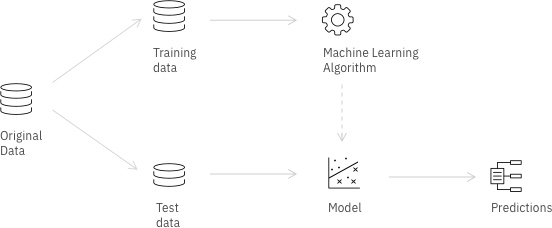
\includegraphics[scale=0.5]{images/ML_Process.jpg}
\caption {Processo padrão para aprendizado de máquina}
\label{fig:MLProcess}
\end{figure}

\item \textbf{Atributo protegido:} São características (\textit{features}) que não podem ser usadas como base para decisões. Geralmente são considerados dados sensíveis, como raça, religião, nacionalidade, sexo, estado civil, idade e status socioeconômico.

\item \textbf{Grupo privilegiado:} Agrupamento de dados relacionados a valores de atributos protegidos que sofrem discriminação e devem ser privilegiados na fase de treinamento para classificar o modelo final como justo.

\item \textbf{Grupo não-privilegiado:} Agrupamento de dados relacionados a valores de atributos protegidos que não sofrem discriminação e devem ser desprivilegiados na fase de treinamento para classificar o modelo final como justo.

\item \textbf{Verdadeiro positivo (TP):} Um caso em que os resultados previstos e reais estão ambos na classe positiva.

\item \textbf{Falso positivo (FP):} Um caso previsto para estar na classe positiva
quando o resultado real pertence à classe negativa.

\item \textbf{Falso negativo (FN):} Um caso previsto para estar na classe negativa
quando o resultado real pertence à classe positiva.

\item \textbf{Verdadeiro negativo (TN):} Um caso em que os resultados previstos e reais estão ambos na classe negativa.

\item \textbf{Regressão Logística}: Algoritmo utilizado em aprendizado de máquina para, em sua variação mais comum, realizar classificação binária de rótulos através de uma função sigmóide. Pode classificar mais de dois rótulos se utilizar a técnica \textit{One-Vs-All} ou utilizar uma variação chamada Regressão Logística multinomial.

\item \textbf{Regularização}: Conjunto de técnicas que tem como objetivo tirar ruídos presentes no processo de aprendizado que podem evitar o modelo final de ser generalizado, acarretando o que é chamado de \textit{Overfitting}

\item \textbf{AI Fairness 360}: Biblioteca para a linguagem Python criada pela IBM que cataloga diversas técnicas de aprendizado de máquina baseados em métricas de Fairness para serem utilizadas. Também encapsula conjuntos de dados com seus grupos protegidos e não-protegidos
\end{itemize}

\section{Métricas}

\subsection{Métricas primitivas}

\begin{itemize}
\item \textbf{Precisão, ou valor preditivo positivo (PPV):} É a fração de casos positivos previstos corretamente para estar na classe positiva de todos os casos positivos previstos no modelo. Ou seja, $PPV = \frac{TP}{TP + FP}$
\item \textbf{Taxa de descoberta falsa (FDR):} É a fração de casos negativos previstos incorretamente como estando na classe positiva de todos os casos positivos previstos no modelo. Ou seja, $FDR  = \frac{FP}{TP + FP}$
\item \textbf{Taxa de falsa omissão (FOR):} É a fração de casos positivos previstos incorretamente como estando na classe negativa de todos os casos negativos previstos no modelo. Ou seja, $FOR = \frac{FN}{TN + FN}$
\item \textbf{Valor preditivo negativo (NPV):} É a fração de casos negativos previstos corretamente para estar na classe negativa de todos os casos negativos previstos no modelo. Ou seja, $NPV = \frac{TN}{TN + FN}$
\item \textbf{Sensibilidade ou \textit{recall}, ou taxa positiva verdadeira (TPR):} É a fração de casos positivos previstos corretamente para estar na classe positiva de todos os casos positivos reais. Ou seja, $TPR = \frac{TP}{TP + FN}$
\item \textbf{Taxa de falsos positivos (FPR):} É a fração de casos negativos previstos incorretamente como estando na classe positiva de todos os casos negativos reais. Ou seja, $FPR = \frac{FP}{FP + TN}$
\item \textbf{Taxa de falsos negativos (FNR):} É a fração de casos positivos previstos incorretamente como estando na classe negativa de todos os casos positivos reais. Ou seja, $FNR = \frac{FN}{TP + FN}$
\item \textbf{Taxa negativa verdadeira (TNR):} É a fração de casos negativos previstos corretamente para estar na classe negativa de todos os casos negativos reais. Ou seja, $TNR = \frac{TP}{FP + TN}$
\end{itemize}

\subsection{Métricas compostas}

\begin{itemize}
\item \textbf{Diferença de paridade estatística, ou discriminação~\citep{Zemel_2013}:} Esta métrica é baseada na seguinte fórmula:

\begin{align*}
Pr(Y=1|D=nao-privilegiado)-Pr(Y=1|D=privilegiado)
\end{align*}
 
Aqui, o viés ou paridade estatística é a diferença entre a probabilidade de que um indivíduo aleatório retirado dos não-privilegiados seja rotulado como 1 e a probabilidade de que um indivíduo aleatório dos privilegiados seja rotulado como 1. Portanto, um valor próximo de 0 é considerado justo.

\item \textbf{Diferença de oportunidade igual:} É a diferença entre a taxa positiva verdadeira do grupo não privilegiado e a taxa positiva verdadeira do grupo privilegiado:

\begin{align*}
TPR_{D=nao-privilegiado} - TPR_{D=privilegiado}
\end{align*}
 
Um valor próximo de 0 é considerado justo, assim como na métrica anterior.

\item \textbf{Diferença de probabilidade média:} Essa métrica usa a taxa de falsos positivos e a taxa positiva verdadeira para calcular a tendência, calculando a igualdade de probabilidades com a fórmula:

\begin{align*}
\frac{1}{2}(|FPR_{D=nao-privilegiado} - FPR_{D=privilegiado}|+|TPR_{D=nao-privilegiado} - TPR_{D=privilegiado}|)
\end{align*}
 
Também precisa ser próximo a 0 para ser considerado justo.

\item \textbf{Impacto de disparidade:} Para esta métrica, é usada a seguinte fórmula:

\begin{align*}
\frac{Pr(Y=1|D=nao-privilegiado)}{Pr(Y=1|D=privilegiado)}
\end{align*}

Usa as mesmas probabilidades da diferença de paridade estatística, mas aqui são calculadas como proporção. Desta forma, um valor próximo de 1 é considerado justo.

\item \textbf{Indíce de Theil:} Esta medida também é conhecida como índice de entropia generalizado, mas com $\alpha$ igual a 1. É calculado com a seguinte fórmula:

\begin{align*}
\frac{1}{n}\sum^{n}_{i=0}\frac{b_i}{\mu}\ln{\frac{b_i}{\mu}}
\end{align*}

Onde $b_i = \hat{y}_i - y_i + 1$, $y_i$ é o conjunto de saídas e $\hat{y}_i$ é o conjunto de previsões dadas pelo modelo. Também precisa ser próximo a 0 para ser considerado justo.

\end{itemize}

\section{Algoritmos}

\subsection{Pré-processamento}

\begin{itemize}
\item \textbf{Reposição (Reweighing)~\citep{Kamiran_2011}:} Pondera os exemplos em cada combinação de grupo e rótulo de maneira diferente para garantir a justiça antes da classificação.

\item \textbf{Removedor de impacto de disparidade (Disparate impact remover)~\citep{Feldman_2015}:} Edita valores de \textit{features} aumentando a justiça de cada grupo enquanto preserva a ordem de classificação dentro dos mesmos.

\item \textbf{Aprendizado de representações justas (LFR, ou Learning fair representations)~\citep{Zemel_2013}:} Encontra uma representação latente que codifica os dados, mas ofusca informações dos atributos protegidos.

\item \textbf{Pré-processamento otimizado~\citep{Calmon_2017}:} Aprende uma transformação probabilística que edita \textit{features} e rótulos nos dados efetuando justiça em cada grupo, distorção individual, garantindo a fidelidade de dados através de restrições.

\end{itemize}

\subsection{Processamento}

\begin{itemize}
\item \textbf{Remoção de viés adversário (Adversarial debiasing)~\citep{Zhang_2018}:} Aprende um classificador que maximiza a precisão e reduz a capacidade de um adversário de depender do atributo protegido nas previsões. Essa abordagem leva a um classificador justo, pois as previsões realizadas pelo classificador não possuem nenhuma informação de discriminação nos grupos.

\item \textbf{Removedor de preconceito (Prejudice remover)~\citep{Feldman_2015}:} Técnica que adiciona no algoritmo escolhido um termo de regularização baseado na discriminação (No caso da biblioteca AI Fairness 360 é usado o programa da publicação, que usa a regressão logística como algoritmo base).

\item \textbf{Meta-Algoritmo para classificações justas (Meta-Algorithm for Fair Classification)~\citep{Celis_2019}:} Aprende um classificador compatível com uma gama grande de métricas de Fairness, sendo prático o suficiente para abrangê-las sem grande perda de performance.

\item \textbf{Justiça por Subgrupos Ricos (Rich Subgroup Fairness)~\citep{Kearns_2018}:} Aprende um classificador que procura equalizar as taxas de falsos positivos e falsos negativos entre os dados que envolvem atributos protegidos, considerados como subgrupos.

\item \textbf{Redução por Gradiente Exponencial (Exponentiated Gradient Reduction)~\citep{Agarwal_2018}:} Aprende um classificador baseado em Gradiente Exponencial que tende a minimizar o erro de uma classificação ponderada.

\item \textbf{Redução por busca em grid (Grid Search Reduction)~\citep{Agarwal_2018}~\citep{Agarwal_2019}:} Aprende um classificador baseado na busca em um grid de valores que tende a minimizar o erro de uma classificação ponderada. É mais simples e impreciso que a Redução por Gradiente Exponencial, mas sua escolha pode ser razoável se a quantidade de métricas de Fairness a serem consideradas for pequena.

\end{itemize}

\subsection{Pós-processamento}

\begin{itemize}
\item \textbf{Igualdade de probabilidade calibrada (Calibrated Equalized odds)~\citep{Pleiss_2017}:} Otimiza as previsões do classificador obtido, calibrando para alterar os rótulos de saída e obter probabilidades igualadas entre os grupos.

\item \textbf{Igualdade de probabilidade (Equalized odds)~\citep{Hardt_2016}:} Resolve um problema linear para alterar os rótulos de saída e obter probabilidades igualadas entre os grupos.

\item \textbf{Classificação baseada em Rejeição de Opções (Reject Option-based Classification)~\citep{Kamiran_2012}:} Dá resultados favoráveis para grupos não privilegiados e resultados desfavoráveis para grupos privilegiados de acordo com uma faixa de confiança.

\end{itemize}

\section{Exemplo de Problema}

\begin{itemize}
\item \textbf{Objetivo:} Obter classificação de crédito (boa ou ruim), através de uma série de \textit{features}

\item \textbf{Conjunto de dados:} German Credit Dataset, presente em \citep{ucigerman_2021}.

\item \textbf{Atributo protegido:} Idade

\item \textbf{Grupo privilegiado:} Idade maior ou igual a 25 anos

\item \textbf{Grupo não-privilegiado:} Idade menor que 25 anos

\end{itemize}

\section{Papeis de pessoas em ML}

\subsection{Diagrama de atividades}

Ver Figura \ref{fig:AIRoles}.

\begin{figure}[h]
\centering
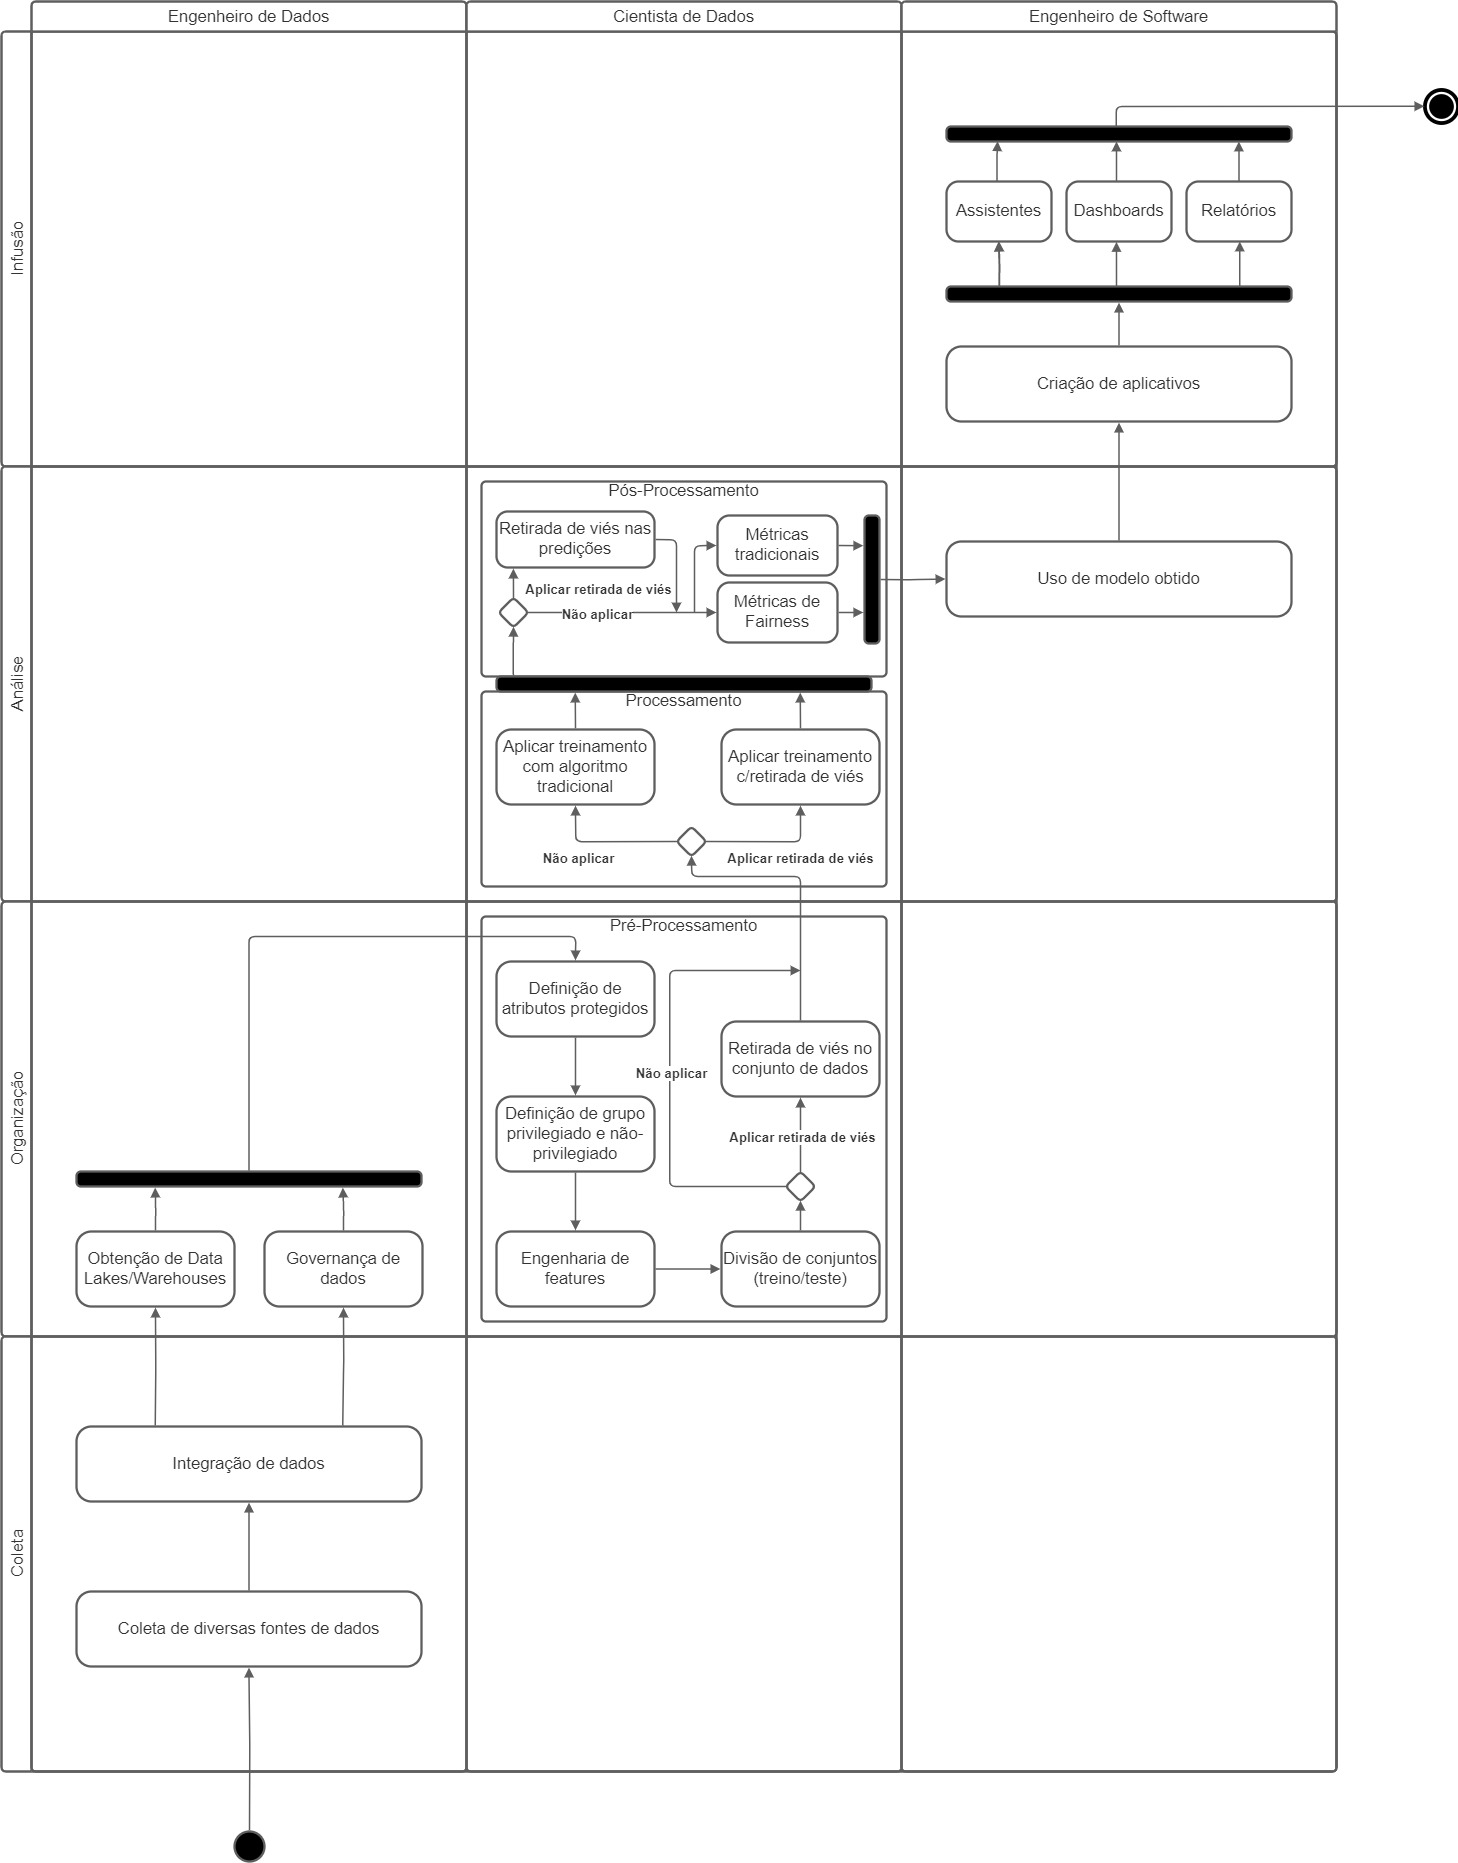
\includegraphics[scale=0.32]{images/Diagrama_Atividades.jpg}
\caption {Diagrama de atividades com subdivisão de cada papel em uma aplicação de IA utilizando métricas de Fairness, com base na IBM AI Reference Architecture~\citep{IBM_2021}}
\label{fig:AIRoles}
\end{figure}

\subsection{Cargos}

\begin{itemize}
\item \textbf{Engenheiro de Dados:} Responsável pela coleta, estruturação, organização, consolidação/integração dos dados em \textit{Data Lakes/Data Warehouses} e processos de governança.

\item \textbf{Cientista de Dados:} Responsável pela análise de dados coletados e estruturados pelo Engenheiro de Dados e criação de processos de ML.

\item \textbf{Engenheiro de Software:} Responsável pelo uso do modelo de ML gerado pelo cientista de dados e desenvolvimento de aplicações para uso geral.

\item \textbf{Cargos Auxiliares:} É possível que outros cargos auxiliem o desenvolvimento destes, como \textit{Product Owners} para entenderem os usos do cliente final e Advogados para determinarem boas práticas aos processos de governança.

\end{itemize}

\subsection{Conteúdo}

\begin{itemize}
\item \textbf{Ambiguidade entre os papeis de Ciência de Dados - Acadêmico:} \url{http://www.ijsrd.com/articles/IJSRDV8I90019.pdf}

\item \textbf{Papel do Cientista de Dados - Acadêmico:} \url{https://dl.acm.org/doi/pdf/10.1145/2884781.2884783}

\item \textbf{Perfis de Cientista de Dados - Acadêmico:} \url{http://www.ijsrd.com/articles/IJSRDV8I90019.pdf}

\item \textbf{Diferença entre Cientista, Analista e Engenheiro de Dados - Miscelâneo:} \url{https://www.geeksforgeeks.org/what-are-the-roles-and-responsibilities-of-a-data-scientist/}
\end{itemize}

\section{Arquitetura Pipes and Filters em ML}

\subsection{Pipes e Filtros}

\begin{itemize}
\item \textbf{Classificação e sequência de Filtros:} Pré-Processamento $>$ Processamento $>$ Pós-Processamento

\item \textbf{Entrada do Pipe para pré-processamento:} Conjunto de dados original

\item \textbf{Filtros para pré-processamento:} Definições de atributos protegidos, Definições de grupos privilegiados e não-privilegiados, Engenharia de features, Divisão de conjuntos, técnicas de aumento/diminuição de dados (oversampling/undersampling) e algoritmos para retirada de vieses no dado.

\item \textbf{Saída do Pipe para pré-processamento:} Conjunto de dados com tratamentos feitos na fase de pré-processamento e divididos para treinamento, validação (recomendável) e testes

\item \textbf{Entrada do Pipe para processamento:} Conjunto de dados com tratamentos feitos na fase de pré-processamento e divididos para treinamento

\item \textbf{Filtros para processamento:} Algoritmos para treinamento, independentemente de ter retirada de vieses ou não.

\item \textbf{Saída do Pipe para processamento:} Modelos obtidos pós-treinamento

\item \textbf{Entrada do pipe para pós-processamento:} Conjunto de dados com tratamentos feitos na fase de pré-processamento e divididos para testes, e modelos obtidos pós-treinamento

\item \textbf{Filtros para pós-processamento:} Algoritmos para retirada de vieses nas predições, cálculo de métricas e escolha de modelo mais adequado.

\item \textbf{Saída do pipe para pós-processamento:} Métricas utilizadas e modelo mais otimizado de acordo com elas.
\end{itemize}

\subsection{Fluent API}

É possível abstrair tal arquitetura através do conceito de Fluent Interface~\citep{Fowler_2005} (também conhecido como Fluent API~\citep{Nakamaru_2020}). Dessa forma, é possível encadear diversos processos que dependem uns dos outros em uma sintaxe mais intuitiva e que procura dar mais clareza ao fluxo dos dados.

Nele, os componentes de filtro representam as operações a modificar e/ou processar os dados, e os componentes de pipes representam os dados presentes no fluxo como um todo. Com ela, é possível com poucas linhas de código transformar um pipe através de um filtro passando componentes como entrada:

\begin{lstlisting}[language=Python, caption=Manipulações de pipes em filtros]
	initial_pipe.to_filter(Filter1())
				.to_pipe(Pipe())
				.to_filter(Filter2())
				.to_pipe(Pipe())
\end{lstlisting}

É possível também criar novos pipes encadeando dados de outros pipes e obtendo parte dos mesmos:

\begin{lstlisting}[language=Python, caption=Conversões de pipes em outros pipes]
	initial_pipe.merge(another_pipe)
				.partial_pipe('prop1', 'prop2')
\end{lstlisting}

Com o uso de métodos especiais presente no Python, é possível mudar alguns operadores para estes objetos com o objetivo de deixar a sintaxe ainda mais simples:

\begin{lstlisting}[language=Python, caption=Facilitando a sintaxe através de métodos especiais]
# Sintaxe equivalente ao encadeamento de pipes com filtros
	initial_pipe >= Filter1() == Pipe() >= Filter2() == Pipe()
	
# Sintaxes equivalentes ao encadeamento de pipes com outros
# e obtencao de pipes parciais
	(initial_pipe + another_pipe)['prop1', 'prop2']
	initial_pipe['prop1'] + another_pipe['prop2']
\end{lstlisting}

É possível definir filtros não apenas para processar dados e uso de algoritmos de ML, mas também processos de visualização dos dados para simplificar a análise, como gráficos ou definir DSLs para obtenção dos dados.

\subsection{Conteúdo}

\begin{itemize}
\item \textbf{Pipes and Filters - Acadêmico:} \url{https://www.researchgate.net/publication/221034471_The_Pipes_and_Filters_Pattern_A_Functional_Parallelism_Architectural_Pattern_for_Parallel_Programming}

\item \textbf{Pipes and Filters - Miscelâneo:} \url{https://www.linkedin.com/pulse/software-architectural-patterns-pipes-filters-lakmal-kankanamge/}

\item \textbf{Pipes and Filters - Miscelâneo:} \url{https://docs.microsoft.com/en-us/azure/architecture/patterns/pipes-and-filters}

\item \textbf{Arquitetando um Pipeline de ML:} \url{https://towardsdatascience.com/architecting-a-machine-learning-pipeline-a847f094d1c7}

\item \textbf{Estrutura de um Pipeline de ML (Pipes and Filters/Composite/DAGs):} \url{https://www.neuraxio.com/blogs/news/how-to-code-neat-machine-learning-pipelines}

\item \textbf{Técnicas para aumentar/diminuir dados - Miscelâneo:} \url{https://dl.acm.org/doi/pdf/10.1145/2884781.2884783}

\end{itemize}

\section{Ataques e segurança}

O \textit{Berryville Institute of Machine Learning} classifica 78 riscos de segurança que uma aplicação baseada em Machine Learning é capaz de sofrer~\citep{McGraw_2020}. Os 10 principais são:

\begin{itemize}
\item \textbf{Exemplos adversários:} São os ataques mais comuns a serem discutidos. A ideia é enganar uma aplicação de Machine Learning fornecendo dados maliciosos, muitas vezes envolvendo pequenas distorções que fazem com que o sistema faça uma previsão ou categorização falsa, por mais que os dados cubram boa parte das situações.

\item \textbf{Envenenamento de dados:} Como um aplicação de Machine Learning aprende diretamente a partir dos dados que possui, os dados desempenham um papel desproporcional na segurança. Se um invasor puder manipular intencionalmente os dados usados de maneira coordenada, todo o modelo pode ser comprometido. Deve-se considerar que fração dos dados de treinamento um invasor pode controlar e até que ponto.

\item \textbf{Manipulação do sistema online:} Uma aplicação de Machine Learning está “online” quando continua a aprender durante o uso operacional, modificando seu comportamento ao longo do tempo. Nesse caso, um invasor inteligente pode empurrar propositalmente o sistema que ainda está aprendendo na direção errada por meio da entrada do sistema e, lentamente, “retreinar” a aplicação para fazer a coisa errada. Esse tipo de ataque pode ser sutil e razoavelmente fácil de executar. Esse risco é complexo, exigindo considerar a proveniência dos dados, a escolha do algoritmo e as operações do sistema.

\item \textbf{Ataque de \textit{Transfer Learning}:} Em muitos casos no mundo real, aplicações de Machine Learning são construídas tirando proveito de um modelo padrão já treinado que é então ajustado para realizar uma tarefa mais específica. Um ataque de transferência de dados ocorre quando tal modelo padrão está comprometido, ou inadequado, tornando possível um comportamento imprevisto definido pelo invasor.

\item \textbf{Confidencialidade dos dados:} Há um grande desafio em proteger dados sensíveis ou confidenciais que, por meio de treinamento, são integrados a um modelo. Ataques de extração sutis desses dados são um risco a ser considerado.

\item \textbf{Confiabilidade dos dados:} Considerar a procedência e a integridade dos dados é essencial. Os dados precisam ser adequados e de qualidade, os sensores confiáveis, e a integridade dos dados deve ser preservada. Compreender a natureza das fontes de dados da aplicação (durante o treinamento e a execução) é de extrema importância. Os riscos de transmissão de dados são particularmente complexos quando se trata de fontes de dados públicas (que podem ser manipuladas ou envenenadas) e modelos online.

\item \textbf{Reprodutibilidade:} Infelizmente, por causa de sua natureza impenetrável e do crescimento rápido do campo, os resultados das aplicações de Machine Learning são frequentemente sub-relatados, mal descritos e, de outra forma, impossíveis de reproduzir. Isso torna o futuro de sua manutenção incerto.

\item \textbf{\textit{Overfitting}:} Quando uma aplicação de Machine Learning "decora" seu conjunto de dados de treinamento, ele não generaliza para novos dados e é considerado \textit{overfitting}. Tais modelos são particularmente fáceis de atacar. O \textit{Overfitting} também é possível em conjunto com a manipulação do sistema online e pode acontecer enquanto um sistema está em execução.

\item \textbf{Integridade da codificação dos dados:} Os dados são frequentemente codificados, filtrados, re-representados e processados de outra forma antes de serem usados (na maioria dos casos por um grupo de pessoas). Problemas de integridade de codificação podem distorcer um modelo de diferentes maneiras. Por exemplo, as codificações que incluem metadados podem permitir que um modelo "resolva" um problema de categorização enfatizando demais os metadados e ignorando o problema real de categorização, podendo acontecer algum tipo de ruído.

\item \textbf{Integridade dos dados de saída:} Se um invasor puder se interpor entre uma aplicação de Machine Learning e seu uso no mundo real, um ataque direto na saída pode ser possível. A natureza impenetrável do modelo final (ou seja, não entender realmente como fazem o que fazem) pode tornar um ataque de integridade de saída muito mais fácil, pois uma anomalia pode ser mais difícil de detectar.
\end{itemize}


\subsection{Possíveis soluções}

\begin{itemize}

\item O AIF360 possui suporte ao ART (\url{https://github.com/Trusted-AI/adversarial-robustness-toolbox}), onde é possível simular ataques

\item Uma outra alternativa é o \url{https://github.com/google-research/robustness_metrics}

\end{itemize}

\subsection{Conteúdo}

\begin{itemize}
\item \textbf{High Quality Machine Learning - Série de 3 artigos:} 
	\begin{itemize}
	\item \url{https://medium.com/codex/high-quality-machine-learning-part-1-d45259ee7613}

	\item \url{https://medium.com/codex/high-quality-machine-learning-part-2-2643c144a2a7}

	\item \url{https://medium.com/codex/high-quality-machine-learning-part-3-c660b885233c}
	\end{itemize}

\item \textbf{Adversarial ML Threat Matrix:} \url{https://github.com/mitre/advmlthreatmatrix}

\item \textbf{Hands-On Guide To Adversarial Robustness Toolbox (ART):} \url{https://analyticsindiamag.com/adversarial-robustness-toolbox-art/}

\end{itemize}



\bibliographystyle{plainnat}
\bibliography{project}
\end{document}
